%===================================== CHAP 2 =================================

\chapter{Problem Description} \label{chapter_problem_description}

This chapter presents the problem description of the thesis. First, the rules and point system of Fantasy Premier League are described in Section \ref{rules of fpl} and Section \ref{point_system}, respectively. The rules and point system are given in correspondence with the information found on FPL's homepage, www.fantasy.premierleague.com. Finally, in Section \ref{section_prob_desc_fpldp}, the \textit{Fantasy Premier League Decision Problem} is formulated. 


\newpar

Before the rules of the FPL and the point system are presented, some terms are defined. First, it is important to make the distinction between a \textit{manager} and a \textit{player} clear. Henceforth, the term manager refers to a participant in the FPL, while player refers to a real-life football player competing in the English Premier League. Furthermore, by football, we always refer to European Football, also known as soccer.


\section{Rules of Fantasy Premier League} \label{rules of fpl}


In order to understand the dynamics of Fantasy Premier League, a review of the game rules is necessary. The Premier League consists of 20 teams and every team faces each other two times during a season. Thus, each season consists of 380 fixtures split into a set of 38 chronological \textit{gameweeks}. In general, every gameweek consists of 10 fixtures featuring each team once. All the matches within a gameweek are usually played over a period of 3-4 days. However, due to matches in the national and international cups, some of the Premier League matches are postponed or played ahead of its original dates. This implies that some of the gameweeks do not consist of exactly 10 fixtures. Gameweeks consisting of more than 10 fixtures are hereby referred to as \textit{double} gameweeks, while gameweeks consisting of less than 10 fixtures are referred to as \textit{blank} gameweeks.


\newpar

Initially, a manager must select a team of 15 players consisting of exactly: 2 goalkeepers, 5 defenders, 5 midfielders and 3 forwards. This is regarded as the \textit{selected squad}. As each team has a registered squad of 25 players, the whole FPL database consists of approximately 500 players. This creates numerous ways of selecting the team. The total purchase price of the team may not exceed the initial budget limit of \pounds 100m. Notice that the budget limit may vary over time, as player prices increase and decrease during the season. Further, one can not select more than 3 players from the same club. After the FPL manager has picked the selected squad, a \textit{starting line-up} consisting of 11 players from the selected squad has to be chosen. A manager can compose the starting line-up in any formation as long as there is exactly 1 goalkeeper, at least 3 defenders, at least 3 midfielders and at least 1 forward. This is regarded as the \textit{team formation criteria}. The players in the starting line-up are the only players that are awarded points. However, if any player from the starting line-up is not playing, he will be replaced by one of the four substitutes on the bench. As only 1 goalkeeper can feature in the starting line-up, the goalkeeper will only be substituted in if the goalkeeper in the starting line-up is not playing. For the remaining 3 substitutes, each manager must set a \textit{substitution priority}, deciding the order of substitution. It is important to note that the formation criteria overrules the substitution priority. Consider a case where you have 3 defenders in your starting line-up and a midfielder with substitution priority 1. If a defender in your starting line-up does not play, the formation criteria ensures that the defender can not be replaced by the midfielder. 

\newpar

Each player in the FPL database is assigned with a price, depending on how well the player is expected to perform. Player prices change during the season depending on the popularity of the player in the transfer market. A player's price will increase when more managers select him, and decrease when fewer managers select him. If the price of a player increases while a manager has the player in the selected squad, the manager can benefit from the price increase. However, if the player is sold, a \textit{sell-on fee} of 50\% is inferred. Hence, the manager only receives 50\% of the profit (rounded down to the nearest \pounds 0.1m). For example, if a manager buys a player for \pounds 9.5m and the player's value increases to \pounds 10.0m in a later gameweek, the manager receives \pounds 9.7m if the player is sold, earning a profit of \pounds 0.2m. Thus, there is a distinction between a player's \textit{value} and \textit{sell price}. A player's value is the price a player is listed with in the FPL database. If a player is \textit{not} in a manager's selected squad, this is the price the manger must pay for the player. A player's sell price is the price a manager can sell a player in the selected squad for. If the price of a player decreases, his sell-price simply equals his value.



\newpar

For each gameweek, managers may use one \textit{free transfer} if they want to replace one of their players in the selected squad  with another player. It is possible to make more than one transfer for a gameweek, but each additional transfer will deduct 4 points from the total score. Hereby, transfers deducting points are referred to as \textit{penalized transfers}. If a manager chooses not to make any transfers for a gameweek, the free transfer is saved for the next gameweek and the manager can make two free transfers in the upcoming gameweek. However, a manager can not save up more than two free transfers. That is, not making any transfers for two consecutive gameweeks does not give the opportunity to make three free transfers in the upcoming gameweek.


\begin{figure}[H]
\centering
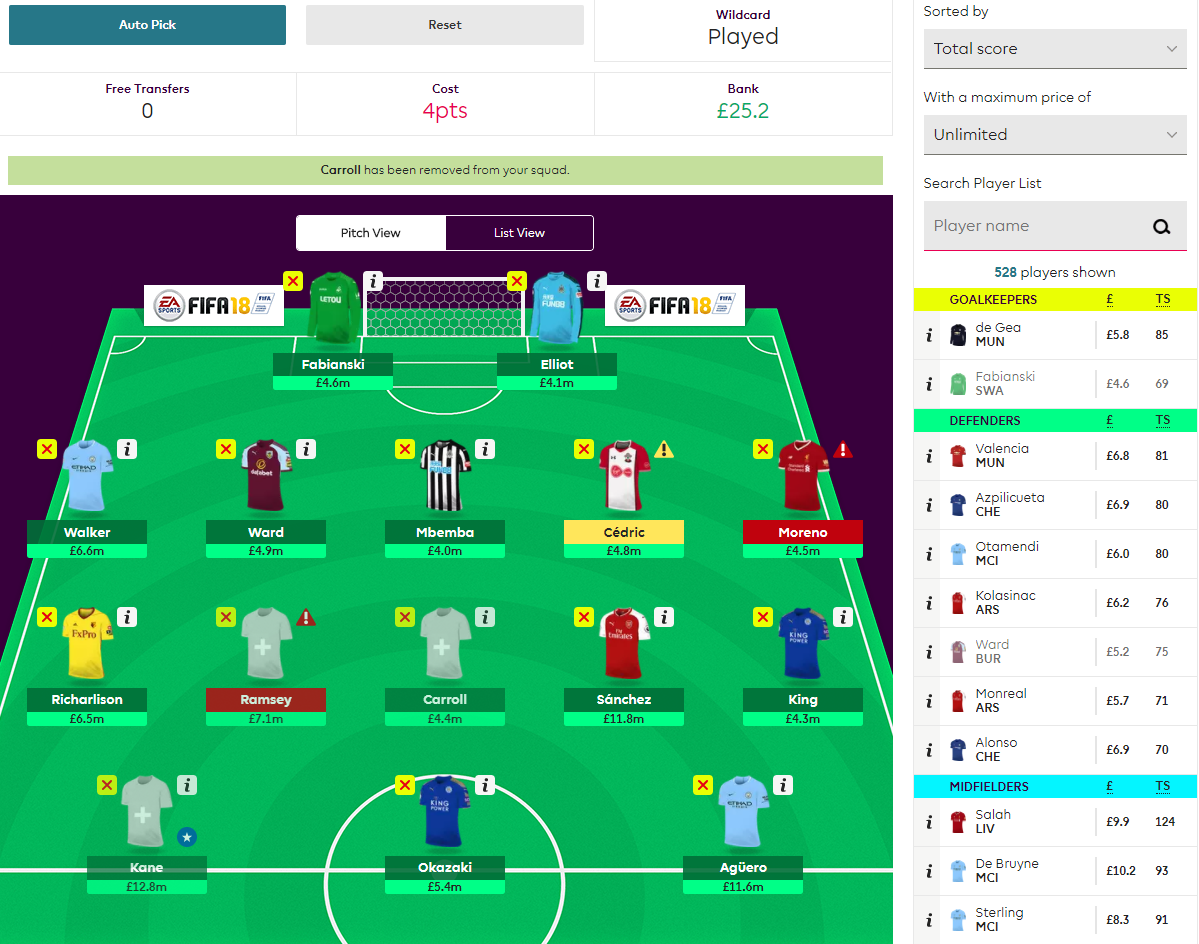
\includegraphics[scale=0.35]{fig/fantasyteam1.png}
 \captionsource{Illustration of the team selection page of Fantasy Premier League.}{\url{https://fantasy.premierleague.com/a/squad/transfers} (10.01.2018)}
\label{Figure_2.1}
\label{fig:fantasy_bilde}
\end{figure}

Figure \ref{Figure_2.1} illustrates how a selected squad is picked in FPL. The grey shirts indicate that the manager is considering to remove Kane, Ramsey and Carroll from the selected squad. As one can see, this deducts 4 points. Hence, the manager had two free transfers for this gameweek. Further, the manager has \pounds 25.2m left in the bank if these transfers are carried out. In addition, it is observed that Ramsey and Moreno have a red triangle attached to them. This implies that they are either injured or suspended for the upcoming gameweek. Notice how the selected squad consists of exactly 2 goalkeepers, 5 defenders, 5 midfielders and 3 forwards as stated in the rules. 


\section{The Point System} \label{point_system}

The Premier League managers are rewarded with points depending on their performance during a gameweek. The main point factors are related to goals scored, assists given and clean sheets. In the following, the point system is presented. 

\begin{table}[H]
\centering
\small
\begin{tabular}{|l|c|c|c|c|}
\hline
                               & Goalkeepers & Defenders & Midfielders & Forwards \\
\hline
For playing up to 60 minutes   & 1           & 1         & 1           & 1        \\
For playing 60 minutes or more & 2           & 2         & 2           & 2        \\
For each goal scored           & 6           & 6         & 5           & 4        \\
For each assist                & 3           & 3         & 3           & 3        \\
For keeping a clean sheet      & 4           & 4         & 1           & -        \\
For every 3 saves made         & 1           & -         & -           & -        \\
For each penalty saved         & 5           & -         & -           & -        \\
For each penalty missed        & -2          & -2        & -2          & -2       \\
For every two goals conceded   & -1          & -1        & -           & -        \\
For each yellow card           & -1          & -1        & -1          & -1       \\
For each red card              & -3          & -3        & -3          & -3       \\
For each own goal              & -2          & -2        & -2          & -2      \\
\hline
\end{tabular}
\caption{Point system of FPL.}
\end{table}

\begin{itemize}
    \item In a match, the three best players are evaluated according to the FPL Bonus Points System, and are awarded a bonus of 1, 2 and 3 points. Bonus Points are calculated according to 32 match statistics, where goals scored, assists and clean sheets are the factors that are heaviest weighted. A complete overview of the Bonus Points System is given in Appendix \ref{A1_BPS}.
    \item In order for a goalkeeper or defender to receive points for a clean sheet, he has to play at least 60 minutes, excluding stoppage time. 
    \item If a goal is scored on a direct free kick or a penalty, the player who got the free kick/penalty is awarded with an assist. 
    \item For each round, a manager chooses a captain and a vice-captain. If the captain is playing, he will be awarded with double points for the entire round. However, if the captain is not playing, the vice-captain will be awarded double points. If neither the captain nor the vise-captain played, no players are given double points.
\end{itemize}


Notice that the point system does \textit{not} consider the outcome of a match. Hence, players are not rewarded with points for playing on a team that wins or loses. In addition to the regular scoring system, each manager is awarded four different gamechips, where only one gamechip can be used in a gameweek: 
\begin{enumerate} [label=(\roman*)]

\item \textbf{Wildcard}. The Wildcard can be used twice a season, once in the first and once in the second half of the season. A Wildcard allows the manager to replace his entire selected squad for free. As for the Wildcard squad selection, the same rules applies as in the regular fantasy team composition. Hence, one can only select a maximum of three players from each team and the formation constraints must be held. When playing a Wildcard, a manager's budget is set to the sell price of his original squad at that particular gameweek. Further, when playing a Wildcard, any saved transfers will be lost. One will be back to the usual 1 free transfer the following gameweek.

\item \textbf{Bench Boost}. The Bench Boost allows you to receive points for all the 15 players of your selected squad. The gamechip can only be used once a season. 

\item \textbf{Free Hit}. The Free Hit allows the manager to replace his entire selected squad for one gameweek. However, for the next gameweek your selected squad from previous gameweek will return. The Free Hit can only be used once a season. As for the Wildcard, the same transfer- and budget rules applies for the Free Hit.

\item \textbf{Triple Captain}. The Triple Captain triples the points of your captain for a gameweek. If the captain does not play, the points of the vice-captain are tripled. The Triple Captain can only be used once a season. If neither the captain nor the vise-captain play, no players are given triple points.
\end{enumerate}

\section{The Fantasy Premier League Decision Problem} \label{section_prob_desc_fpldp}

In Fantasy Premier League each manager attempts to maximize his or her total number of points over an entire season. As seen in this chapter, a number of decisions must be made each gameweek. The decisions considers which players to include in the selected squad and which players to pick for the starting line-up. In addition, a captain- and vice-captain must be chosen. Further, one has to set a substitution priority for the players that are not selected for the starting line-up. As pointed out, a manager is allowed to perform transfers during the season. Therefore, a manager must also decide whether to make a transfer or not, and consequently which players to be transferred in and out for each gameweek. Hence, decisions are made in a multi-period manner. Hereby, the aforementioned decisions are referred to as the Fantasy Premier League Decision Problem (FPLDP).